\chapter{Конструкторская часть}
В данном разделе будут указаны требования к ПО, реализованы схемы алгоритмов сортировок и будут приведены рассчеты трудоемкостей для этих алгоритмов.

\section{Требования к ПО}
К программе предъявлен ряд требований:
\begin{itemize}
    \item входными данными являются две матрицы, каждя из которых хранится в файле, с расширением \texttt{*.txt};
    \item результат выполнения программы~--- матрица, полученная в результате умножения введенных матриц;
    \item возможность произвести замеры процессорного времени выполнения реализованных алгоритмов.
\end{itemize}

\section{Разработка алгоритмов}
На рисунке \ref{fig:Stand} представлена схема алгоритма для стандартного умножения.

На рисунках \ref{fig:Vinograd1}--\ref{fig:Vinograd2} представлены схемы алгоритма умножения методом Винограда.

На рисунках \ref{fig:VinogradOpt1}--\ref{fig:VinogradOpt2} представлены схемы оптимизированного алгоритма умножения методом Винограда.

\begin{figure}[h]
	\centering
	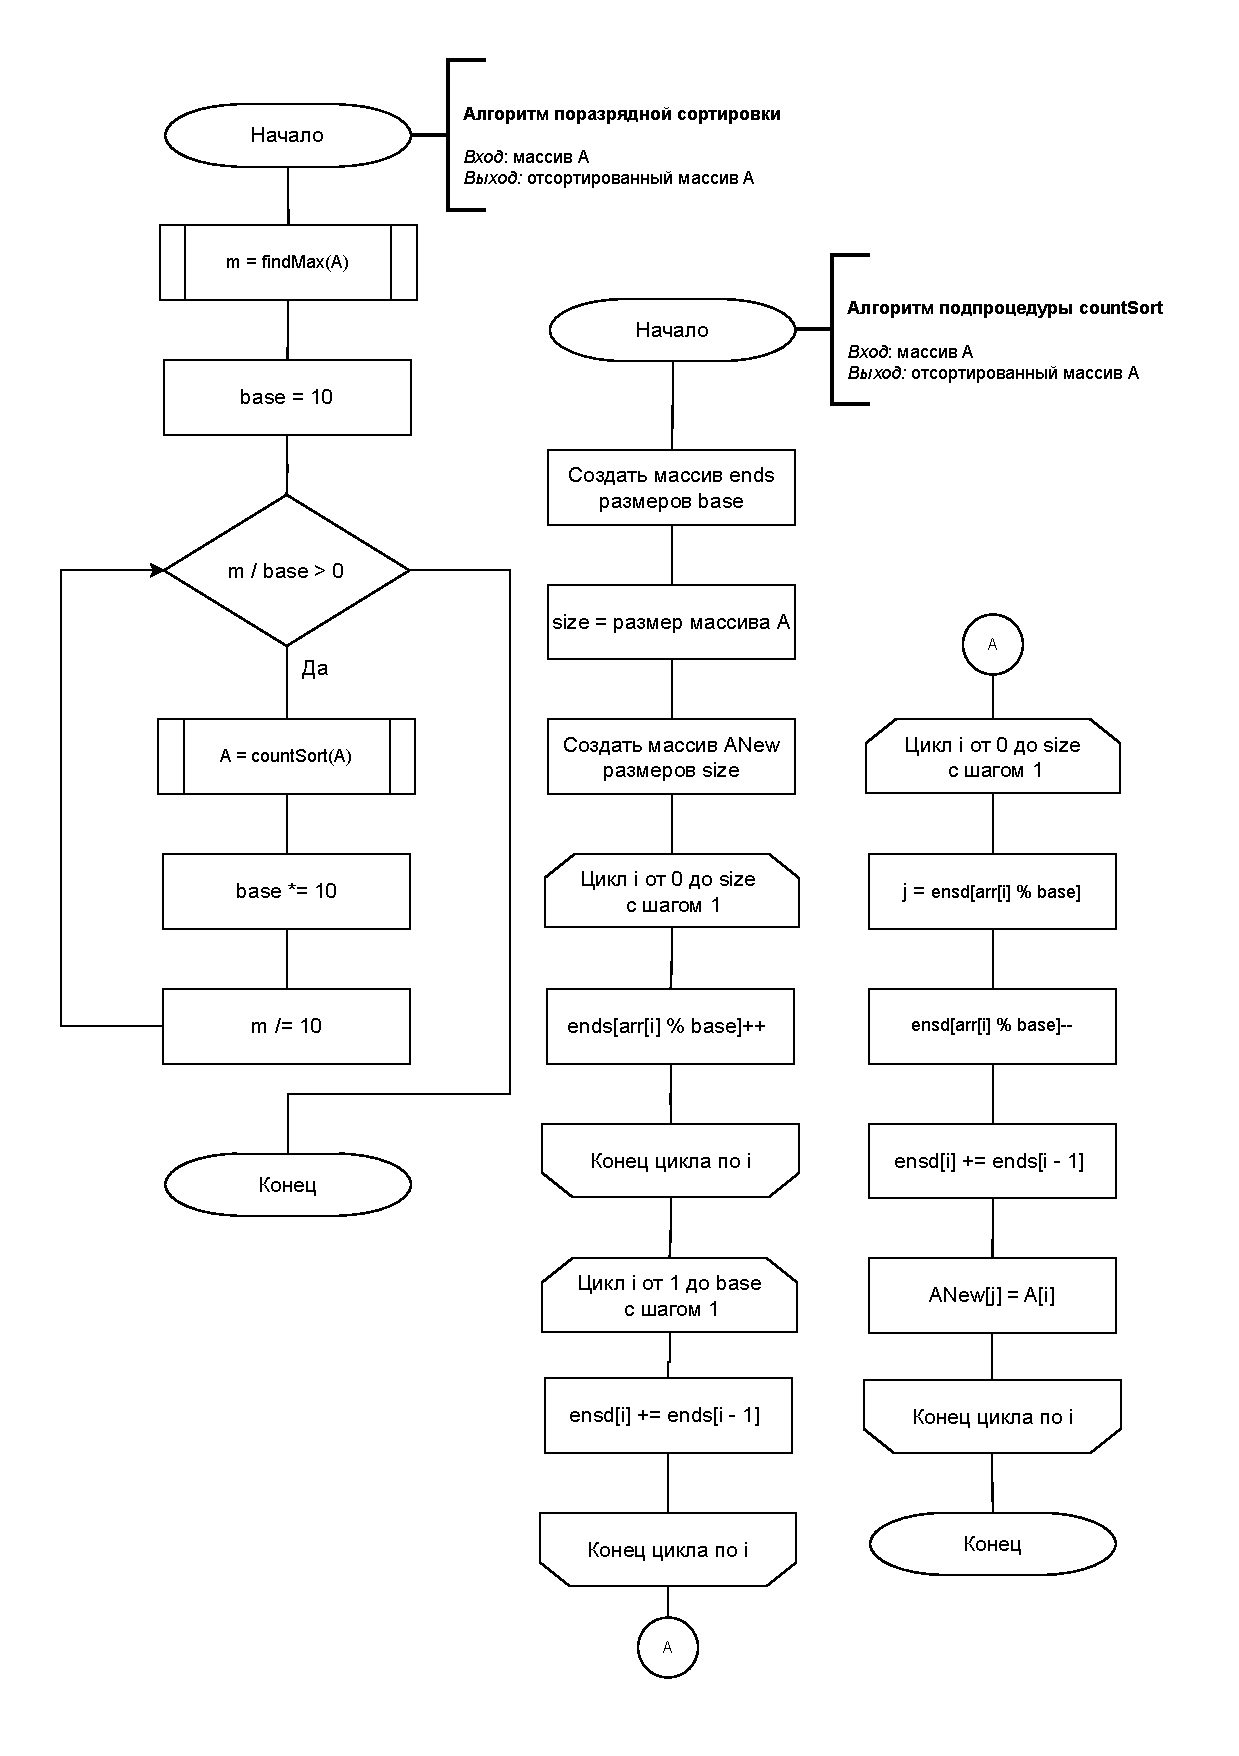
\includegraphics[height=0.9\textheight, page=1]{img/algorithms.pdf}
	\caption{Схема стандартного алгоритма умножения матриц}
	\label{fig:Stand}
\end{figure}

\clearpage

\begin{figure}[h]
	\centering
	\includegraphics[height=0.9\textheight, page=2]{img/algorithms.pdf}
	\caption{Схема алгоритма умножения матриц методом Винограда (начало)}
	\label{fig:Vinograd1}
\end{figure}

\clearpage

\begin{figure}[h]
	\centering
	\includegraphics[height=0.9\textheight, page=3]{img/algorithms.pdf}
	\caption{Схема алгоритма умножения матриц методом Винограда (конец)}
	\label{fig:Vinograd2}
\end{figure}

\clearpage

\begin{figure}[h]
	\centering
	\includegraphics[height=0.9\textheight, page=4]{img/algorithms.pdf}
	\caption{Схема оптимизированного алгоритма умножения матриц методом Винограда (начало)}
	\label{fig:VinogradOpt1}
\end{figure}

\clearpage

\begin{figure}[h]
	\centering
	\includegraphics[height=0.9\textheight, page=5]{img/algorithms.pdf}
	\caption{Схема оптимизированного алгоритма умножения матриц методом Винограда (конец)}
	\label{fig:VinogradOpt2}
\end{figure}

\clearpage

\section{Модель вычислений для проведения оценки трудоемкости алгоритмов}
Для последующего вычисления трудоемкости необходимо ввести модель вычислений:

\begin{enumerate}
	\item операции из списка \ref{eq:operations1} имеют трудоемкость \textbf{1};
	\begin{equation}
		\label{eq:operations1}
		\begin{gathered}
			+, -, =, +=, -=, ==, !=, <, >, <=, >=, [], \\ ++, --, \&\&, >>, <<, ||, \&, |
		\end{gathered}
	\end{equation}
	\item операции из списка \ref{eq:operations2} имеют трудоемкость \textbf{2};
	\begin{equation}
		\label{eq:operations2}
		*, /, \%, *=, /=, \%=
	\end{equation}
	\item трудоемкость условного оператора \texttt{if условие then A else B} рассчитывается как \ref{eq:if};
	\begin{equation}
		\label{eq:if}
		f_{if} = f_{\text{условия}} + 
		\begin{cases}
			f_{A}, & \text{в случае выполнеия условия,}\\
			f_{B}, & \text{иначе}.
		\end{cases}
	\end{equation}
	\item трудоемкость цикла рассчитывается как \ref{eq:for}
	\begin{equation}
		\label{eq:for}
		\begin{gathered}
			f_{for} = f_{\text{инициализация}} + f_{\text{сравнения}} + M_{\text{итераций}} \cdot (f_{\text{тело}} +\\
			+ f_{\text{инкремент}} + f_{\text{сравнения}});
		\end{gathered}
	\end{equation}
	\item трудоемкость вызова функции равна 0.
\end{enumerate}

\section{Трудоемкость алгоритмов}
В следующих частях будут приведены рассчеты трудоемкостей алгоритмов для умножения матриц.

\subsection*{Поразрядная сортировка}

\subsection*{Сортировка расческой}

\subsection*{Сортировка Шелла}

\section*{Вывод}
В данном разделе были указаны требования к ПО, а также на основе теоретических данных, полученных в аналитическом разделе, были построены схемы алгоритмов сортировок. Оценены трудоемкости в лучшем и худшем случаях. 